\documentclass[11pt]{article}
\usepackage[utf8]{inputenc}
\usepackage[english]{babel}
\usepackage{graphicx}         % For including images
\usepackage{amsmath, amssymb, amsfonts}          % For mathematical notation
\usepackage[margin=2cm]{geometry}  % Margins
\usepackage[font=normalsize,labelfont=small]{caption}  % Caption style
\usepackage{hyperref}
% For clickable links
\usepackage{booktabs}
\usepackage{multicol}
\usepackage{subcaption}

\usepackage{bm}                 % \bm for bold vectors and matrices
\usepackage{enumitem}           % list control (e.g. [nosep] in itemize)


\usepackage{float}
\usepackage{tabularx}
\usepackage{array}
\usepackage{setspace}


% MAXIMUM LENGTH: 5 PAGES WITHOUT EXCEPTION.
\begin{document}
\onehalfspacing

\begin{titlepage}
    \centering
    \vspace*{2cm}
    
\includegraphics[scale=1.8]{Logo-Udesa.jpg}\par
    \vspace{10pt}

    {\LARGE \textbf{I302 - Machine Learning\\ and Deep Learning}\par}
    \vspace{1cm}

    {\LARGE \textbf{Final Project: \\Anomaly Detection in ECG Signals}\par}
    \vspace{4cm}

    {\LARGE {Ana Paula Tissera and Naomi Couriel}\par}  % <- Modify Name and Surname
    \vspace{4cm}

    {\Large July 2, 2025\par}
    \vspace{1cm}
    \Large{Artificial Intelligence Engineering}
\end{titlepage}

% ABSTRACT
\begin{abstract}

In this work we address the problem of automatic anomaly detection in ECG signals, with the goal of assisting clinical diagnosis. To this end, we developed a hybrid pipeline composed of a 1D Variational Autoencoder (VAE) and an XGBoost classifier, fed by the VAE latent representation and its reconstruction error. The model is trained exclusively on normal records from the PTB-XL and Chapman-Shaoxing databases, using lead II segments and morphological coefficients extracted through an FMM model. We evaluate the system with standard metrics (AUC, Precision, Recall, F1, Accuracy) on an unseen test set, obtaining an AUC of 0.81 and, at an operating point chosen for high recall, a Recall of 0.74 and a Precision of 0.71. The results validate the approach and motivate improvements such as attention mechanisms or data augmentation.

\end{abstract}

% INTRODUCTION
\section{Introduction}


Cardiovascular diseases are one of the leading causes of mortality worldwide, and the electrocardiogram (ECG) is the most widely used non-invasive tool for their diagnosis. However, its manual analysis is slow, costly and dependent on specialists, hindering its large-scale application. This work addresses anomaly detection in ECG signals, seeking to automatically filter out normal records from those that require clinical review.

We propose a two-stage hybrid pipeline that combines unsupervised and supervised learning, using records from the public PTB-XL and Chapman-Shaoxing databases. The input to the system are 2048-sample lead II segments, together with a vector of 21 morphological coefficients (FMM). The output is a binary classification: \textit{Normal} or \textit{Anomalous}.

First, we train a convolutional 1D Variational Autoencoder (VAE) on normal segments, using lead II and 2048-sample windows, complemented with FMM coefficients that characterize the morphology of the P, Q, R, S and T waves. In this context, anomalies produce high reconstruction errors relative to healthy signals.

Then, we combine the encoder latent vectors with the reconstruction error to train an XGBoost classifier that refines the binary decision. The VAE architecture consists of a convolutional encoder with temporal-reduction blocks and a symmetric decoder. The loss includes the reconstruction MSE and the KL divergence, which regularizes the latent space.

This approach leverages the VAE's ability to model the typical variability of normal ECGs, adding XGBoost's precision, and offers a robust and scalable solution for automating ECG analysis.


\section{Dataset and features}
For the development of this work we used two public, open-source ECG databases: PTB-XL and Chapman-Shaoxing. Combining both allowed us to have a diverse and large dataset to train and validate our model.

\subsection{Data Sources}
The PTB-XL dataset contains 21,837 12-lead ECG records (10s at 500 Hz) from 18,885 patients. We follow the data splits recommended by the dataset authors \cite{wagner2020ptb}. The Chapman-Shaoxing dataset contributes 10,646 additional records with similar characteristics \cite{zheng2020chapman}, which we split 80/20 into development and test.

A point that turns out to be decisive: each ECG recording is segmented into several heartbeats (about 7 on average), and every beat is one sample. Splitting those samples at random would put beats of the same patient on both sides of a split, letting the model memorise a patient during training and then be scored on that same patient. \textbf{All splits in this work -- development/test and train/validation -- are therefore grouped by recording}, so that every beat of a recording stays on the same side. With 7 beats per recording, a random beat-level split would leave roughly 80\% of the recordings straddling both sides, and the resulting validation scores are optimistic by a wide margin (in our own runs, validation AUC dropped from $0.91$ to $0.85$ once the grouping was enforced). After the split, the development set holds 20,907 recordings and the test set 3,254, with no recording in common.

\subsection{Preprocessing and Feature Extraction} \label{sec: Preprocesamiento}

The signal preprocessing and morphological coefficient extraction in this work are based on the methodology developed in the FMM-Head repository~\cite{verardo2023fmmhead}, which provides datasets already segmented, filtered and annotated with the parameters of the FMM model. Specifically, we use the \texttt{ptb\_xl\_fmm} and \texttt{shaoxing\_fmm} versions, which contain the ECG signal already centered on R peaks, cropped to 2048 samples and accompanied by a vector of 21 coefficients per beat.

Following the approach of the original repository, lead II signals are selected because their recording axis ($\sim$+60°) coincides with the natural direction of atrial and ventricular depolarization, facilitating the clear identification of the P wave (atrial depolarization), the QRS complex (ventricular depolarization) and the T wave (ventricular repolarization), whose changes in shape or duration, such as anomalies in QRS width or T-wave inversion, may indicate ischemia or conduction blocks, among others. These signals are then passed through a low-pass filter to remove baseline drift caused by breathing or movement.

Next, R peaks are detected using the Pan-Tompkins equations and the RR interval is defined as the time difference between successive R peaks. Each beat is segmented centered on the R peak, taking 40\% of the previous RR interval and 60\% of the following one, and is zero-padded up to a fixed length of 2048 samples (a multiple of the \textit{batch size}) to feed the model.

The shape of each beat is described using the Frequency Modulated Möbius (FMM) model, which approximates the signal as the sum of five modulated waves (P, Q, R, S and T):
\vspace{-0.5em}
\[
x(t) \;=\; \sum_{j=1}^{5} A_j \,\sin\!\Bigl(\omega_j t \;+\;\beta_j\,\arctan\!\bigl(\tan\bigl(\tfrac{t-\alpha_j}{2}\bigr)\bigr)\Bigr) \;+\; C,
\]
\vspace{-0.1em}
where \(A_j\) is the amplitude, \(\omega_j\) the frequency, \(\alpha_j\) the central phase, \(\beta_j\) the asymmetry parameter and \(C\) a global offset. In this way, each wave contributes five parameters and the offset adds one, giving a total of 21 morphological coefficients. To avoid angular discontinuities, each phase \(\alpha_j\) is encoded as \(\bigl(\cos\alpha_j,\;\sin\alpha_j\bigr)\), and all parameters are ordered according to the corresponding wave, from P to T \cite{verardo2023fmmhead}.

The signal modulated from this sum captures the essential shape of each beat, preserving the features relevant for anomaly detection -as evidenced in Figures \ref{fig:sano_comparacion} and \ref{fig:anomalo_comparacion} - and, at the same time, provides a more informative representation to the model.


\vspace{0.5em}


% --- Healthy signal figures ---
\begin{figure}[ht]
    \centering
    \begin{subfigure}[b]{0.43\textwidth}
        \centering
        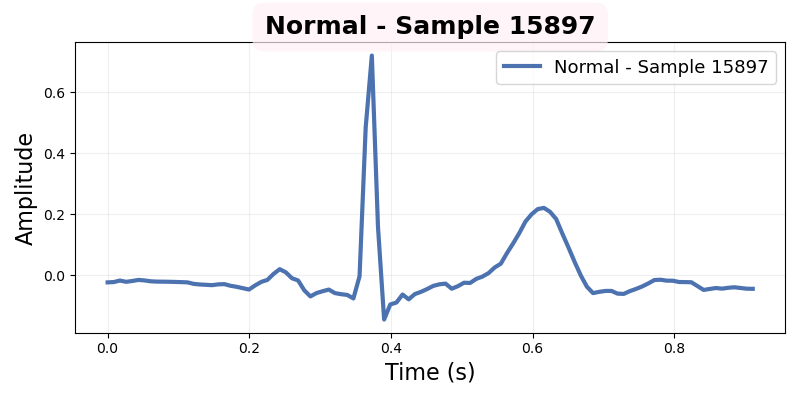
\includegraphics[width=\textwidth]{Graficos/Visualizacion/senal_sana.png}
        \caption{Healthy signal}
        \label{fig:senal_sana}
    \end{subfigure}
    \hfill
    \begin{subfigure}[b]{0.43\textwidth}
        \centering
        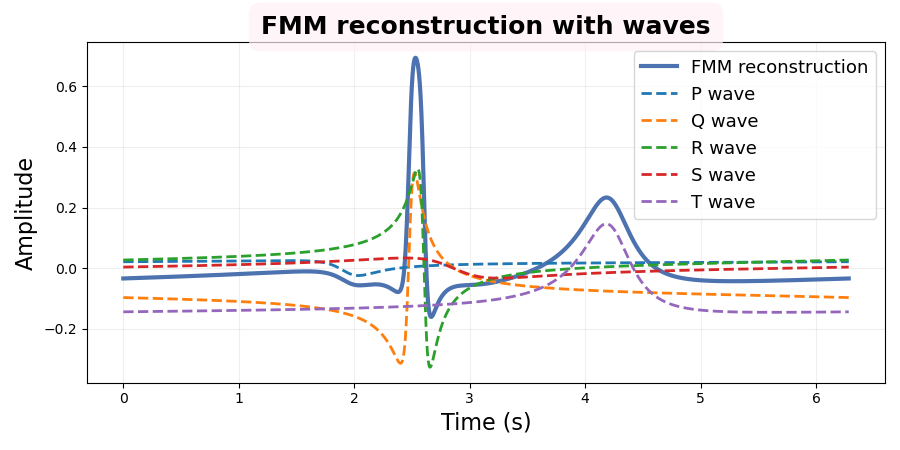
\includegraphics[width=\textwidth]{Graficos/Visualizacion/FMM_sano.png}
        \caption{Healthy FMM}
        \label{fig:fmm_sano}
    \end{subfigure}
    \caption{Comparison between a healthy signal and its FMM reconstruction.}
    \label{fig:sano_comparacion}
\end{figure}


% --- Anomalous signal figures ---
\begin{figure}[ht]
    \centering
    \begin{subfigure}[b]{0.43\textwidth}
        \centering
        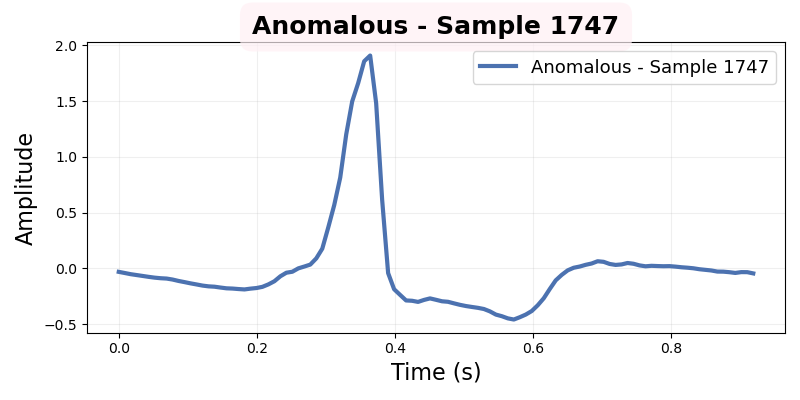
\includegraphics[width=\textwidth]{Graficos/Visualizacion/senal_anomala.png}
        \caption{Anomalous signal}
        \label{fig:senal_anomala}
    \end{subfigure}
    \hfill
    \begin{subfigure}[b]{0.43\textwidth}
        \centering
        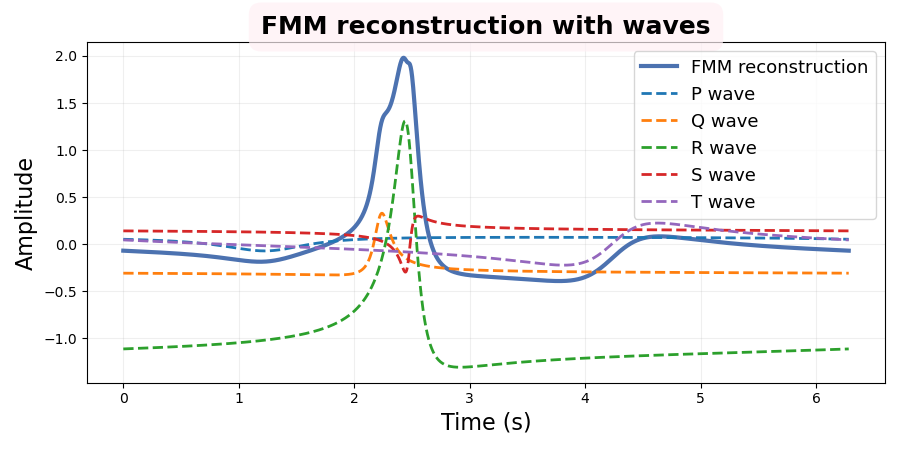
\includegraphics[width=\textwidth]{Graficos/Visualizacion/FMM_anomalo.png}
        \caption{Anomalous FMM}
        \label{fig:fmm_anomalo}
    \end{subfigure}
    \caption{Comparison between an anomalous signal and its FMM reconstruction.}
    \label{fig:anomalo_comparacion}
\end{figure}

\newpage


In addition, this 21-feature vector is used as a conditional input to the VAE together with the modulated ECG signal. In this way, the VAE not only learns to reconstruct based on the signal, but also does so based on the explicit morphological features, improving its representation capacity.

Finally, to avoid information leakage between sets, we compute the mean and standard deviation exclusively over the normal windows of the training set. These values were used to standardize all windows (training, validation and test) to zero mean and unit variance, thus guaranteeing the integrity of the validation process.



% METHODS
\section{Methodology}

In this section we describe in detail the algorithms that make up our hybrid pipeline: the convolutional 1D Variational Autoencoder (VAE) and the supervised XGBoost classifier.


\subsection{Conditional 1D Variational Autoencoder}

The VAE is defined as a probabilistic generative model with an \textit{encoder}
\(
q_\phi(\mathbf{z} \mid \mathbf{x}_s, \mathbf{x}_f)
\)
and a \textit{decoder}
\(
p_\theta(\mathbf{x}_s \mid \mathbf{z}).
\)
The \textit{encoder} processes the ECG signal $\mathbf{x}_s$ and the FMM coefficient vector $\mathbf{x}_f$ to map them to a latent distribution. Its architecture is as follows:
\vspace{-0.2em}
\begin{itemize}
    \item An initial layer $\mathrm{Conv1D}(1\to32,\; k=19,\; s=2,\; p=9)$ with $\mathrm{LeakyReLU}$ activation.
    \vspace{-0.2em}
    \item $n_{\mathrm{blocks}}=2$ 1D residual blocks
    \(
       \mathrm{ResBlock1D}(32,\; k=3,\; \mathrm{dilation} = 1,2,4)
    \)
    that use increasing dilations to enlarge the receptive field without altering the temporal resolution.
    \vspace{-0.2em}
    \item A \textit{flatten} of the convolutional output, which is concatenated with the FMM coefficient vector. %$\mathbf{x}_f$.
    \vspace{-0.2em}
   \item Two dense layers that project the concatenated vector to obtain the parameters of the latent distribution: the mean $\boldsymbol{\mu}$ and the log-variance $\log\boldsymbol{\sigma}^2$, both of dimension $d_z=64$.
\end{itemize}

Through the reparameterization trick, the latent vector $\mathbf{z} = \boldsymbol{\mu} + \boldsymbol{\sigma} \odot \boldsymbol{\epsilon}$ is sampled, with $\boldsymbol{\epsilon} \sim \mathcal{N}(0, I)$.


\noindent The \textit{decoder} reconstructs the signal $\hat{\mathbf{x}}_s$ from $\mathbf{z}$ with a symmetric architecture.


The minimized loss function is the \textit{Evidence Lower Bound} (ELBO):
\vspace{-0.4em}
\begin{equation}
\mathcal{L}_{\mathrm{VAE}} = \mathbb{E}_{q_\phi(\mathbf{z}|\mathbf{x})}[\|\mathbf{x}_s - \hat{\mathbf{x}}_s\|_2^2] + \beta \cdot D_{KL}\bigl(q_\phi(\mathbf{z}|\mathbf{x}) \parallel \mathcal{N}(0,I)\bigr)
\end{equation}
\vspace{-0.2em}
where the first term is the reconstruction error (MSE) and the second the Kullback-Leibler divergence, weighted by the hyperparameter $\beta$.

\vspace{-0.1em}

\subsection{XGBoost Classifier}
Once the VAE is trained, a feature vector $\mathbf{c} = [\boldsymbol{\mu}, e] \in \mathbb{R}^{65}$ is extracted for each signal, where $\boldsymbol{\mu}$ is the latent vector and $e$ the reconstruction error. This vector is used to train an XGBoost classifier that makes the final prediction (\textit{Normal} vs. \textit{Anomalous}).

To convert the continuous XGBoost probabilities into binary labels a decision threshold is needed. Youden's point (maximum sensitivity plus specificity minus one) weighs both errors equally, which does not match the clinical setting: letting an anomalous recording pass as normal is worse than raising a false alarm that a specialist then discards. We therefore select the highest threshold that still reaches a recall of at least $0.80$ on the anomalous class, and we select it on the \textbf{validation} split, which is disjoint from the data used to fit the VAE and the classifier. Choosing it on the training data would bias the operating point optimistically.

\subsection{Evaluation Metrics}
The classifier's performance was evaluated with the following standard metrics for binary classification:

\begin{multicols}{2}
\vspace{-0.5em}
\setlength{\itemsep}{0.2em}
\begin{itemize}
     \item \textbf{Confusion Matrix}: allows visualizing the distribution of cases into true positives (TP), false positives (FP), true negatives (TN) and false negatives (FN), providing a direct representation of the model's behavior.
    \begin{table}[H]
    \centering
    \scriptsize
    \label{tab:confusion_example}
    \begin{tabular}{|l|p{1.45cm}|p{1.45cm}|}
        \hline
         & \textbf{Predicted:\ Positive} & \textbf{Predicted:\ Negative} \\ \hline
        \textbf{Actual: Positive} & TP & FN \\ \hline
        \textbf{Actual: Negative} & FP & TN \\ \hline
    \end{tabular}
    \end{table}

    \item \textbf{Accuracy}: measures the proportion of correct predictions over the total number of samples, defined as
    \begin{equation}
        \textstyle \text{Accuracy} = \frac{TP + TN}{TP + TN + FP + FN} \label{accuracy}
    \end{equation}

    \item \textbf{Precision}: the model's ability not to label a normal sample as anomalous. It is computed as
    \vspace{-0.5em}
    \begin{equation}
        \textstyle P = \frac{TP}{TP + FP}
    \end{equation}

    \item \textbf{Recall (Sensitivity)}: the model's ability to find all anomalous samples. It is computed as
    \vspace{-0.5em}
    \begin{equation}
        \textstyle R = \frac{TP}{TP + FN}
    \end{equation}

    \item \textbf{Precision-Recall Curve}: shows recall on the horizontal axis and precision on the vertical axis as the decision threshold varies; it serves to visualize the trade-off between both metrics and to choose the optimal threshold.

    \item \textbf{F1 Score}: combines precision and recall into a single balanced metric.
    \vspace{-0.5em}
    \begin{equation}
        \textstyle F_1 = 2 \cdot \frac{P \cdot R}{P + R} \label{eq: F-score}
    \end{equation}

    \item \textbf{ROC Curve}: a plot of the TPR (True Positive Rate) against the FPR (False Positive Rate) as the decision threshold varies; it allows visualizing the trade-off between detecting true positives and avoiding false positives.
    \label{met: ROC}

    \item \textbf{AUC-ROC}: the area under the ROC curve, obtained by trapezoidal integration over the relationship between TPR and FPR; it measures the ability to distinguish between classes at different thresholds.

\end{itemize}

\vspace{-0.5em}

\end{multicols}


\vspace{1em}
% RESULTS
\section{Experiments, Results and Discussion}

In this section we present the experimental setup, the selection of actual hyperparameters, the metrics used and the results in both validation and the final test set, together with an error analysis.

\subsection{Experimental setup and hyperparameter selection}
To find the optimal VAE configuration, a hyperparameter sweep was performed, training each combination for 15 epochs. The criterion was to maximize the AUC of the resulting XGBoost classifier on the validation set. The explored ranges were:
\begin{itemize}
    \item Regularization $\beta\in\{1.0, 4.0, 10.0\}$.
    \item Learning rate $\ell_r\in\{10^{-3}, 5\times10^{-4}, 10^{-4}\}$.
    \item Latent dimension $d_z\in\{16, 32, 64\}$.
    \item Number of convolutional blocks $n_{\mathrm{blocks}}\in\{2, 3\}$.
\end{itemize}
The Adam optimizer was used with a \textit{batch size} of 64. The best configuration was $\beta=1.0$, $\ell_r=5\times10^{-4}$, $d_z=64$ and $n_{\mathrm{blocks}}=2$. Because the gap between the top configurations turned out to be smaller than the run-to-run variation of retraining the same configuration (std $\approx 0.009$ AUC over three seeds), the ranking is dominated by noise; we therefore did not enlarge the grid. The model was trained for 35 epochs with these parameters.

\subsection{Data Exploration and FMM Features}
The pipeline in this work incorporates as prior knowledge a set of 21 morphological features extracted through a Fourier-Based Model (FMM). This model, proposed by Verardo et al. (2023), analyzes the morphology of each beat to characterize the P, Q, R, S and T waves as explained in Section \ref{sec: Preprocesamiento}.
These coefficients are fed into the VAE \textit{encoder} to condition the learning of the latent representation.

\vspace{3em}
\subsection{Training Convergence Analysis}
To validate the stability of the unsupervised learning component, the evolution of the VAE loss function was analyzed during its final retraining of 35 epochs. Figure~\ref{fig:loss_curve} shows a smooth and sustained decrease of the total loss (ELBO), as well as of its reconstruction (MSE) and regularization (KL) components. This indicates a stable convergence, with no signs of instability or divergence, which gives confidence in the quality of the features extracted by the VAE.

\begin{figure}[ht!]
    \centering
    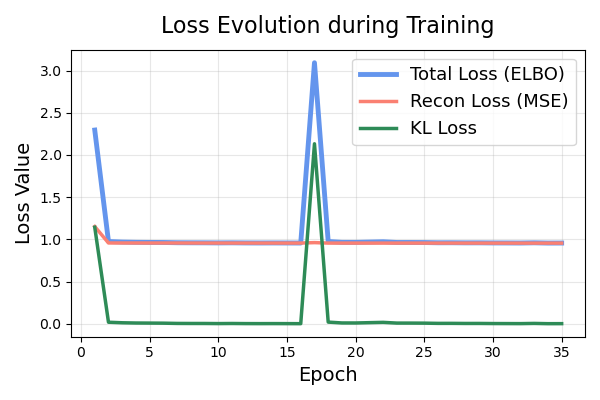
\includegraphics[width=0.55\linewidth]{Graficos/Metricas/TrainLoss.png}
    \caption{VAE loss curves during the 35 epochs of final training. A relatively stable convergence is observed.}
    \label{fig:loss_curve}
\end{figure}

\vspace{-1em}

\subsection{Results on validation and final test}
The numerical results of the final model are summarized in Table~\ref{tab:metrics_comp}. The model reaches an AUC of 0.81 on the held-out test set and 0.91 on validation.

\begin{table}[ht]
  \centering
  \caption{Metrics on validation and final test}
  \label{tab:metrics_comp}
  \begin{tabular}{lcc}
    \toprule
    Metric      & Validation & Final test \\
    \midrule
    AUC-ROC     & 0.8503     & 0.8058     \\
    Precision   & 0.7399     & 0.7116     \\
    Recall      & 0.8001     & 0.7400     \\
    F1-score    & 0.7688     & 0.7255     \\
    Accuracy    & 0.7594     & 0.7200     \\
    \bottomrule
  \end{tabular}
\end{table}

To avoid bias towards the majority class, the test set was balanced through \textit{undersampling}, equalizing the number of normal and anomalous segments.

The confusion matrices (Figure~\ref{fig:cms}) allow visualizing the distribution of errors. On the test set the model correctly identified 4471 anomalous segments and missed 1571 (Recall 0.74), while 1812 normal segments were flagged as anomalous (Precision 0.71). The operating point is deliberately shifted towards recall: for a screening tool a missed anomaly is more costly than a false alarm.

\begin{figure}[ht]
  \centering
  \begin{subfigure}[b]{0.35\textwidth}
    \centering
    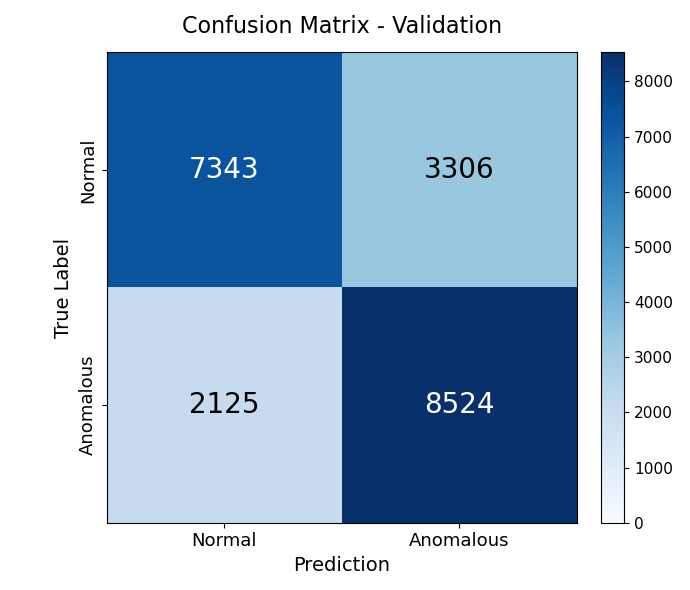
\includegraphics[width=\textwidth]{Graficos/Metricas/CM_tr_val.png}
    \caption{Validation}
  \end{subfigure}
  \quad
  \begin{subfigure}[b]{0.35\textwidth}
    \centering
    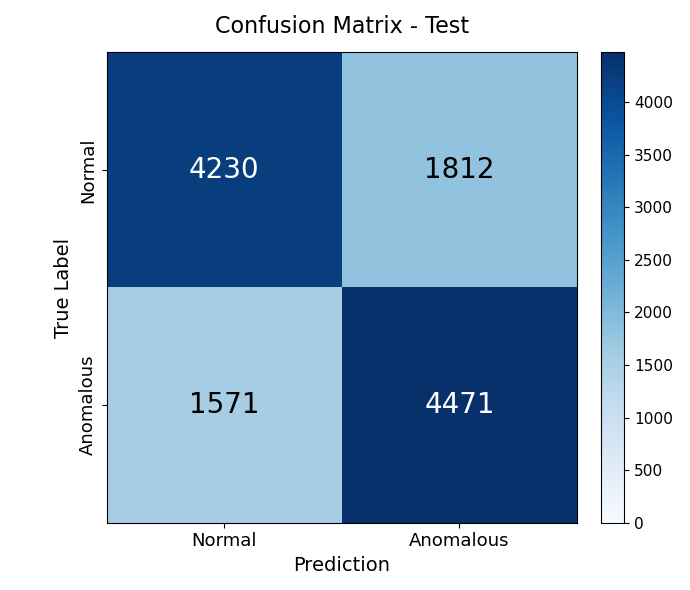
\includegraphics[width=\textwidth]{Graficos/Metricas/CM_dev_test.png}
    \caption{Final test}
  \end{subfigure}
  \caption{Confusion matrices on validation and final test.}
  \label{fig:cms}
\end{figure}

\vspace{4.65em}
On the validation split the recall-constrained rule yielded a threshold of $0.389$, which attains a recall of $0.800$ there. The very same threshold is then applied unchanged to the held-out test set, where it yields a recall of $0.740$: the operating point transfers well but not perfectly, which is expected when moving to recordings from unseen patients.

\begin{figure}[ht!]
    \centering
    \begin{subfigure}[b]{0.45\textwidth}
        \centering
        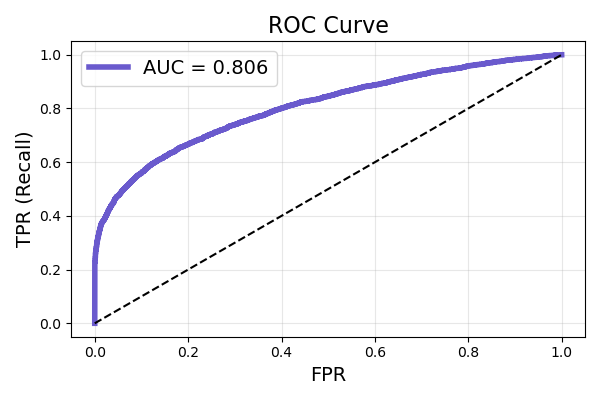
\includegraphics[width=\linewidth]{Graficos/Metricas/ROC_dev_test}
        \caption{ROC Curve (Test)}
    \end{subfigure}
    \hfill
    \begin{subfigure}[b]{0.45\textwidth}
        \centering
        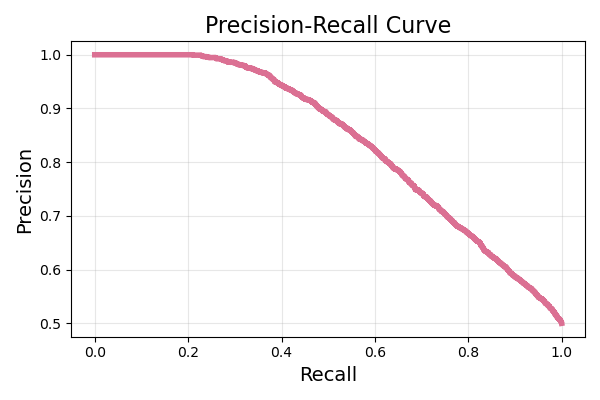
\includegraphics[width=\linewidth]{Graficos/Metricas/PR_dev_test.png}
        \caption{Precision-Recall Curve (Test)}
    \end{subfigure}
    \caption{Performance curves on the test set. The area under the ROC curve (left) confirms the model's good classification ability.}
    \label{fig:curves}
\end{figure}

\vspace{-0.5em}

The ROC and Precision-Recall (PR) curves of the test set (Figure~\ref{fig:curves}) show that the model maintains good discriminative power, with an AUC of 0.8058, well above a random classifier.



\subsection{Discussion}
\vspace{-0.4em}

\subsubsection*{Quantitative analysis}
The hybrid VAE\(+\)XGBoost pipeline surpasses a threshold based solely on reconstruction. On the held-out test set it reaches an AUC of 0.8058, against 0.8503 on validation. Both splits are grouped by recording, so neither number is inflated by seeing other beats of the same patient during training, and the small remaining gap reflects the genuine difficulty of generalizing to new recordings. At the chosen operating point the model recovers 74\% of the anomalous beats at a precision of 0.71; the residual errors are concentrated on the subtler anomalies, whose morphology departs only slightly from a normal beat.

\section{Conclusion and future work}
This behavior reflects a trade-off between Precision and Recall: the model behaves conservatively. Techniques such as attention mechanisms or synthetic augmentation could be explored to improve the ability to detect subtle anomalies. Likewise, more aggressive preprocessing could reduce the impact of noisy signals. Overall, the proposed approach offers a solid foundation, and paves the way towards improvements in robustness against signal and noise variations, proving to be a promising tool to assist the automatic analysis of ECGs in real clinical settings.




\begin{thebibliography}{9}



\bibitem{verardo2023fmmhead}
Giacomo Verardo, Magnus Boman, Samuel Bruchfeld, Marco Chiesa, Sabine Koch, Gerald Q. Maguire Jr., and Dejan Kostic.
\textit{FMM-Head: Enhancing Autoencoder-based ECG anomaly detection with prior knowledge}, 2023.

\bibitem{jang2021unsupervised}
Jong-Hwan Jang, Tae Young Kim, Hong-Seok Lim, and Dukyong Yoon.
\textit{Unsupervised feature learning for electrocardiogram data using the convolutional variational autoencoder}.
PLOS ONE, vol. 16, no. 12, p. e0260612, 2021.
\url{https://doi.org/10.1371/journal.pone.0260612}

\bibitem{wagner2020ptb}
Patrick Wagner, Nico Strodthoff, Robert Bousseljot, Daniel Kreiseler, Frank Lunze, Wojciech Samek, and Thomas Schaeffter.
\textit{PTB-XL: A Large Publicly Available ECG Dataset}. Scientific Data, 7, 154 (2020).
\url{https://doi.org/10.1038/s41597-020-0495-6}

\bibitem{zheng2020chapman}
Jie Zheng, Jinbo Zhang, Sibao Danioko, et al.
\textit{A 12-lead electrocardiogram database for arrhythmia research covering more than 10,000 patients}. Scientific Data, 7, 48 (2020).
\url{https://doi.org/10.1038/s41597-020-0381-4}

\bibitem{pytorch}
Paszke, A., Gross, S., Massa, F., Lerer, A., Bradbury, J., Chanan, G., ... \& Chintala, S. (2019).
\textit{PyTorch: An Imperative Style, High-Performance Deep Learning Library}. NeurIPS.

\bibitem{xgboost}
Chen, T., \& Guestrin, C. (2016).
\textit{XGBoost: A Scalable Tree Boosting System}. Proceedings of the 22nd ACM SIGKDD.

\bibitem{sklearn}
Pedregosa, F., Varoquaux, G., Gramfort, A., Michel, V., Thirion, B., Grisel, O., ... \& Duchesnay, E. (2011).
\textit{Scikit-learn: Machine Learning in Python}. Journal of Machine Learning Research, 12, 2825-2830.

\bibitem{numpy}
Harris, C. R., Millman, K. J., van der Walt, S. J., Gommers, R., Virtanen, P., Cournapeau, D., ... \& Oliphant, T. E. (2020).
\textit{Array programming with NumPy}. Nature, 585(7825), 357-362.

\bibitem{pandas}
McKinney, W. (2010).
\textit{Data Structures for Statistical Computing in Python}. Proceedings of the 9th Python in Science Conference.

\bibitem{matplotlib}
Hunter, J. D. (2007).
\textit{Matplotlib: A 2D graphics environment}. Computing in Science \& Engineering, 9(3), 90-95.

\end{thebibliography}

\subsection*{Data sources}

\begin{enumerate}
  \item \textbf{PTB‑XL ECG Dataset, version 1.0.3.}
    Patrick Wagner et al. (2020). \emph{PTB-XL: A Large Publicly Available ECG Dataset}. \emph{Scientific Data}. Available on PhysioNet: \url{https://doi.org/10.13026/kfzx-aw45}. Cited as \cite{wagner2020ptb}.

  \item \textbf{Chapman‑Shaoxing 12-lead ECG Database.}
    Jie Zheng et al. (2020). \emph{A 12-lead electrocardiogram database for arrhythmia research covering more than 10,000 patients}. \emph{Scientific Data}. Cited as \cite{zheng2020chapman}.

  \item \textbf{Preprocessed FMM (Fast Multi‑resolution Matching) datasets.}
    Publicly available files:
    \begin{itemize}
      \item \url{https://drive.google.com/uc?id=1nYRvbVYJJXPbCwKEqOIeCLnMXdIDAka7}
      \item \url{https://drive.google.com/uc?id=1FjvmVb8-PnpDdoBwv-Eqb89tYFOCx9KW}
    \end{itemize}
    (These files contain the original signals transformed through FMM)
\end{enumerate}


\end{document}
